% ===================================================================
% CertiCut --- Physical Review A (Regular Article) version
% REVTeX 4.2, aps/pra, two-column reprint layout.
%
% The underlying science, theorems, and data are unchanged; the narrative
% is reordered so that the representation-sensitivity question and the
% quasiprobability resource semantics lead, with solver/backend and
% polyhedral engineering moved to the appendices.
%
% Section selection (submission form): A-2E Quantum Information Science.
% PhySH concepts (submission form, not typeset here):
%   Quantum information; Quantum computation; Quantum algorithms;
%   Quantum information processing; Optimization; Numerical methods.
% ===================================================================
\pdfminorversion=7  % allow inclusion of PDF v1.7 figures without warnings
\documentclass[
  aps,
  pra,
  reprint,
  amsmath,
  amssymb,
  longbibliography,
  nofootinbib,
  floatfix
]{revtex4-2}

\usepackage{amsfonts}
\usepackage{amsthm}
\usepackage{booktabs}
\usepackage{placeins}
\usepackage{graphicx}
\usepackage[hidelinks]{hyperref}
\hypersetup{
  pdftitle={Representation Dependence of Optimal Cut Placement in Quasiprobability Circuit Cutting},
  pdfauthor={Phung Trong Hung and Huong Bui},
  pdfsubject={Quantum circuit cutting and quasiprobability resource optimization}
}

\graphicspath{{figures/}}

% Float-placement hygiene: allow more floats per page so the many appendix
% tables/figures do not get stuck, and soak up unbreakable inline math into
% the column gutter rather than overflowing the margin.
\setcounter{topnumber}{5}
\renewcommand{\topfraction}{0.95}
\setcounter{bottomnumber}{5}
\renewcommand{\bottomfraction}{0.95}
\setcounter{totalnumber}{8}
\renewcommand{\textfraction}{0.05}
\renewcommand{\floatpagefraction}{0.80}
\setcounter{dbltopnumber}{5}
\renewcommand{\dbltopfraction}{0.95}
\renewcommand{\dblfloatpagefraction}{0.80}
\emergencystretch=3em

% Let columns end at their natural height instead of stretching rubber glue
% to force a flush bottom. On float-heavy pages this removes the large blank
% gaps that \flushbottom otherwise injects below top floats (e.g. Table IV)
% and around subsection breaks that fall under a wide figure.
\raggedbottom

% Theorem-like environments (plain style: bold header, italic body),
% independent counters so Theorem/Proposition/Corollary each number 1,2,...
\theoremstyle{plain}
\newtheorem{theorem}{Theorem}
\newtheorem{proposition}{Proposition}
\newtheorem{corollary}{Corollary}
% Suppress the QED box (kept from the source: it was mistaken for a
% missing-glyph square in the original build).
\renewcommand{\qedsymbol}{}

\newcommand{\OPT}{\mathrm{OPT}}
\newcommand{\LB}{\mathrm{LB}}
\newcommand{\UB}{\mathrm{UB}}
\newcommand{\gap}{\Delta}

% Table sizing: use a single consistent, natural font size (\footnotesize)
% instead of \resizebox, which would distort each table to a different scale.
% REVTeX's default \tabcolsep is already compact, so it is left untouched.
\newcommand{\tabfit}[1]{{\footnotesize #1}}
\newcommand{\tabfitscript}{\relax}
\newcommand{\tabfitstar}[1]{{\footnotesize #1}}

\begin{document}

\title{Representation Dependence of Optimal Cut Placement in Quasiprobability Circuit Cutting}

\author{Phung Trong Hung}
\email[Contact author: ]{phungtronghung0808@gmail.com}
\affiliation{Faculty of Information Technology, Ho Chi Minh City University of Technology (HUTECH), Ho Chi Minh City, Vietnam}

\author{Huong Bui}
\email{bd.huong@hutech.edu.vn}
\affiliation{Faculty of Information Technology, Ho Chi Minh City University of Technology (HUTECH), Ho Chi Minh City, Vietnam}

\date{\today}

% ===================================================================
% MSC2020 CLASSIFICATION
% ===================================================================
% MSC 2020: 05C85 (Graph algorithms), 68Q25 (Analysis of algorithms and problem complexity), 
%           90C11 (Mixed integer programming), 81P68 (Quantum computation and quantum information)

% ===================================================================
% ABSTRACT
% ===================================================================
\begin{abstract}
Circuit cutting assigns a sampling cost to two-qubit interactions that cross fragment boundaries. Two gate-level representations of the same logical circuit can be unitary-equivalent while inducing different interaction costs, so the placement that minimizes cutting overhead need not remain optimal after a representation change. A direct comparison of one optimizer-returned solution from each representation is unreliable when either problem has multiple optima. We therefore compare complete optimal-placement sets and define the cross-representation regret as the excess log-overhead, in a target representation, of the best placement that was optimal in the source representation. We prove an $\ell_1$ perturbation bound, a sufficient stability condition, and invariance under positive rescaling of all interaction weights. On semantically verified quantum phase-estimation benchmarks, the optimal placement changes under representation conversion; an $n=14$ instance gives an overhead ratio $R=729$. Conversely, six apparent quantum-Fourier-transform reversals disappear when the full optimal sets are compared. For a fixed representation, the independent gate-level quasiprobability-decomposition (QPD) objective reduces exactly to capacitated weighted graph partitioning in the log domain, allowing standard global optimization bounds to be expressed directly as multiplicative overhead bounds. These results show that circuit representation can change the resource-optimal cut placement even when the logical unitary and feasible fragment space are unchanged.
\end{abstract}

\maketitle

% ===================================================================
% I. INTRODUCTION
% ===================================================================
\section{Introduction}
\label{sec:intro}

Near-term quantum processors remain limited in qubit count, fidelity, and connectivity~\cite{preskill2018}. Circuit cutting addresses the width constraint by replacing selected nonlocal operations with combinations of fragment-local operations and reconstructing the target quantity by classical post-processing~\cite{peng2020,bravyi2016,tang2021}. In quasiprobability-based gate cutting, each severed two-qubit interaction contributes a gate-dependent sampling factor. The total overhead is multiplicative, so two placements with the same number of cuts can have very different costs.

The same logical circuit can also have several gate-level representations. Basis translation or decomposition can preserve the unitary up to global phase while changing the two-qubit gates that appear on each pair of logical wires. Under a gate-dependent QPD model, the corresponding interaction weights therefore change. The question studied here is whether that change can move the resource-minimizing cut placement when the logical wires, fragment count, and capacity constraints are held fixed.

There is a subtle degeneracy issue. If representation $a$ has several optimal placements, a solver may return one that is suboptimal under representation $b$ even though another $a$-optimal placement is also optimal under $b$. Comparing one returned solution from each representation can therefore create a false representation effect. We avoid this by comparing the complete optimal-placement sets. Section~\ref{sec:rep} defines the resulting cross-representation regret, proves an $\ell_1$ perturbation bound and a sufficient stability condition, and identifies positive rescaling of all interaction weights as an invariant case.

\begin{figure*}[tp]
  \centering
  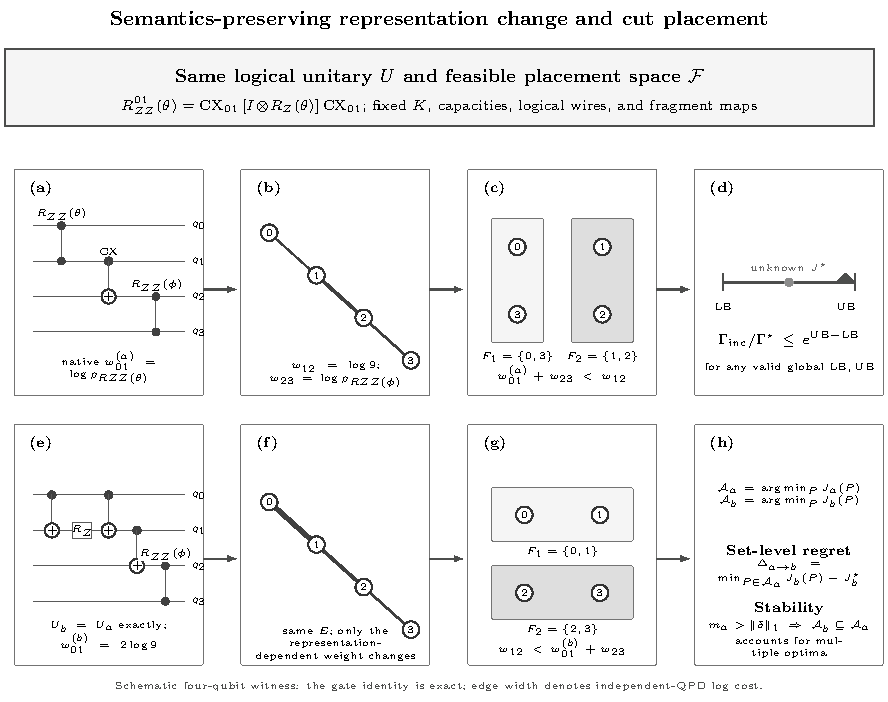
\includegraphics[width=0.86\textwidth]{fig_certicut_architecture.pdf}
  \caption{A four-qubit example of the mechanism studied in this work. Panels (a)--(d) show representation $a$, its weighted interaction graph, an optimal balanced bipartition, and the translation of valid log-objective bounds into an overhead ratio. Panels (e)--(h) replace $R_{ZZ}^{01}(\theta)$ by the exact identity $\mathrm{CX}_{01}[I\otimes R_Z(\theta)]\mathrm{CX}_{01}$. The logical unitary, logical wires, and feasible partition space are unchanged, while the independent-QPD weight on edge $(0,1)$ changes from $\log\rho_{RZZ(\theta)}$ to $2\log 9$. For the displayed edge-weight ordering, this changes the optimal balanced bipartition. Panel (h) shows the set-level comparison used to avoid arbitrary optimizer tie breaking.}
  \label{fig:architecture}
\end{figure*}

The numerical study verifies semantic equivalence before comparing representations. Exact-QPE benchmarks contain strict placement changes, including an $n=14$ instance for which transporting a native-QPD-optimal placement to the CX-normalized representation increases the modeled overhead by a factor of $729$. In contrast, six large QFT regrets obtained by comparing one solver-selected optimum from each representation vanish when the complete optimal sets are compared. These two outcomes provide positive and negative tests of the same set-level criterion.

For a fixed representation, the independent gate-level QPD objective is a capacitated weighted graph-partitioning problem in the log domain. This reduction supplies the optimization model used in the experiments and gives a direct interpretation of valid global lower and upper bounds: if $\LB\leq\OPT\leq\UB$, then the incumbent overhead is at most $\exp(\UB-\LB)$ times the modeled optimum. The graph-partitioning and mixed-integer machinery itself is standard~\cite{deza1997,lawler1966,kaibel2008}.

Our question differs from work that searches a richer cut space for a fixed circuit. Brandhofer \emph{et al.}~\cite{brandhofer2024} optimize mixed gate and wire cuts, Nakamura \emph{et al.}~\cite{nakamura2025} study scalable multi-fragment partitioning and sampling bounds, and Fr{\"o}hler \emph{et al.}~\cite{frohler2026} consider gate, wire, and joint gate-group cuts. Here the fragment space is fixed and the circuit representation changes. The primary cost model is the independent gate-level QPD model implemented by Qiskit Addon Cutting~0.10.0~\cite{qiskitcutting}; joint decompositions, wire cuts, routing, hardware noise, and end-to-end device execution are outside that optimization model. Supporting tests of model sensitivity, finite-shot behavior, backend performance, and interval verification are separated from the central representation result.

% ===================================================================
% II. MODEL
% ===================================================================
\section{Circuit cutting and representation-dependent quasiprobability costs}
\label{sec:model}

\subsection{Independent-QPD circuit cutting}

Gate cutting replaces selected two-qubit channels by quasiprobability decompositions (QPDs) over fragment-local channels~\cite{peng2020,mitarai2021}. For a cuttable channel $\mathcal{U}_g=\sum_i a_{g,i}\mathcal{E}_{g,i}$, the corresponding independent sampling overhead is
\begin{equation}
  \rho_g = \left(\sum_i |a_{g,i}|\right)^{\!2}.
  \label{eq:gate-overhead}
\end{equation}
For a partition $P$ with crossed-gate set $S(P)$, independent sampling across gates gives
\begin{equation}
  \Gamma(P) = \prod_{g \in S(P)} \rho_g, \qquad
  J(P) = \log \Gamma(P) = \sum_{g \in S(P)} \log \rho_g.
  \label{eq:objective}
\end{equation}
This objective matches the independent gate-level model in Qiskit Addon Cutting~0.10.0~\cite{qiskitcutting}; it is not a model of joint decompositions, finite-shot variance, or hardware noise. Because the QPD coefficient one-norm is at least one, $\rho_g\geq1$ and all log weights are nonnegative. We validated the gate costs against the Qiskit QPD registry: $\rho_{\mathrm{CX}}=\rho_{\mathrm{CZ}}=9$, $\rho_{\mathrm{iSWAP}}=\rho_{\mathrm{DCX}}=49$, $\rho_{\mathrm{CS}}=3+2\sqrt{2}\approx5.828$, and $\rho_{RZZ(\theta)}=(1+2|\sin\theta|)^2$ for numerically bound rotations.

\subsection{Log-domain interaction graph}

Let $V=\{0,\ldots,n{-}1\}$ be the circuit qubits, and let $G_{ij}$ contain the two-qubit gate occurrences acting on pair $(i,j)$. We assign the nonnegative interaction weight
\begin{equation}
  w_{ij} = \sum_{g \in G_{ij}} \log \rho_g.
  \label{eq:weight}
\end{equation}
For any fragment map $f:V\rightarrow\{1,\ldots,K\}$, the objective becomes
\begin{equation}
  J(P) = \sum_{i < j} w_{ij} \cdot \mathbb{I}(f(i)\neq f(j)).
  \label{eq:graph-objective}
\end{equation}
The binary bisection identity $\mathbb{I}(f(i)\neq f(j))=|z_i-z_j|$ is recovered when $K=2$.

\begin{proposition}[Objective equivalence]\label{prop:obj-equiv}
Under independent gate-level QPD, minimizing~\eqref{eq:objective} is equivalent to minimizing~\eqref{eq:graph-objective}.
\end{proposition}
\begin{proof}
Every $g\in G_{ij}$ is cut exactly when $f(i)\neq f(j)$. Regrouping the gate-level sum by qubit pair yields~\eqref{eq:graph-objective}.
\end{proof}

\subsection{Representation changes and the common edge universe}
\label{sec:rep-changes}

For the semantics-preserving transformations considered here, basis translation and native-gate decomposition produce circuits implementing the same unitary up to global phase while altering the two-qubit interaction multigraph, and hence the weights~\eqref{eq:weight}. Let $a$ and $b$ be two semantically equivalent representations of the same logical circuit on the same logical wire set $V$, with interaction edge sets $E_a$ and $E_b$. We define the common edge universe $E=E_a\cup E_b$ and zero-pad the log-weights, $w^{(a)}_e=0$ for $e\notin E_a$ and $w^{(b)}_e=0$ for $e\notin E_b$, so that both representations are compared over a single feasible partition space. Because the paired representations share the same logical wire set and declared capacity constraints, the same partition map is feasible for both within the supported independent-QPD model; only the induced interaction weights change. Section~\ref{sec:rep} makes precise the sense in which a change from $a$ to $b$ can move the optimal placement.

% ===================================================================
% III. REPRESENTATION THEORY
% ===================================================================
\section{Representation-sensitive optimal cut placement}
\label{sec:rep}

\subsection{Cross-representation regret over optimal sets}
\label{sec:set-regret}

Consider the fixed logical qubit set $V=\{0,\ldots,n{-}1\}$ evaluated over a common feasible partition space $\mathcal{F}$ defined by a fixed fragment count $K$ and capacity bounds. For any partition $P\in\mathcal{F}$, the log objectives of the two representations are $J_a(P)=(w^{(a)})^\top z(P)$ and $J_b(P)=(w^{(b)})^\top z(P)$, where $z(P)\in\{0,1\}^{|E|}$ is the cut-indicator vector over the common edge universe $E$ of Sec.~\ref{sec:rep-changes}. Let $\mathcal{A}_a=\arg\min_{P\in\mathcal{F}}J_a(P)$ and $J_b^*=\min_{P\in\mathcal{F}}J_b(P)$. We define the set-level cross-representation regret and corresponding sampling-overhead ratio by
\begin{equation}
  \Delta_{a\to b} = \min_{P \in \mathcal{A}_a} J_b(P) - J_b^*, \qquad R_{a\to b} = \exp(\Delta_{a\to b}).
  \label{eq:regret}
\end{equation}
The minimum over $\mathcal{A}_a$ reports positive regret only when every $a$-optimal placement is suboptimal under $b$. When $R_{a\to b}=1$, at least one optimal partition under representation $a$ remains optimal under $b$ ($\mathcal{A}_a\cap\mathcal{A}_b\neq\varnothing$). When $R_{a\to b}>1$, every optimal partition under $a$ is strictly suboptimal under $b$. In general $R_{a\to b}\neq R_{b\to a}$.

\subsection{Representation-regret bound}

The following perturbation statements are exact model-level results; the medium-tier numerical evaluations of Sec.~\ref{sec:results} are solver-tolerance quantities. Let $\delta=w^{(b)}-w^{(a)}\in\mathbb{R}^{|E|}$ be the interaction-weight perturbation vector over the edge universe $E$.

\begin{proposition}[Representation-regret bound]\label{prop:regret-bound}
For any common feasible partition space $\mathcal{F}$, $0\le\Delta_{a\to b}\le\|\delta\|_1$, and $R_{a\to b}\le\exp(\|\delta\|_1)$.
\end{proposition}
\begin{proof}
Let $P_a\in\arg\min_{P\in\mathcal{A}_a}J_b(P)$ and $P_b\in\mathcal{A}_b$. Then $J_b(P_a)-J_b(P_b)=[J_a(P_a)-J_a(P_b)]+\delta^\top[z(P_a)-z(P_b)]$. Because $P_a$ is $J_a$-optimal, $J_a(P_a)-J_a(P_b)\le0$. Since $\|z(P_a)-z(P_b)\|_\infty\le1$, we obtain $\Delta_{a\to b}\le|\delta^\top[z(P_a)-z(P_b)]|\le\|\delta\|_1$.
\end{proof}

\subsection{Stability theorem and scaling invariance}

Let $m_a=\min_{P\in\mathcal{F}\setminus\mathcal{A}_a}[J_a(P)-J_a^*]$ denote the optimality margin of representation $a$, with the convention $m_a=+\infty$ if $\mathcal{F}\setminus\mathcal{A}_a=\emptyset$. Define $m_b$ analogously for representation $b$.

\begin{theorem}[Representation stability]\label{thm:stability}
If $m_a>\|\delta\|_1$, then $\mathcal{A}_b\subseteq\mathcal{A}_a$, and consequently $R_{a\to b}=1$.
\end{theorem}
\begin{proof}
For any $P\in\mathcal{A}_a$ and $Q\in\mathcal{F}\setminus\mathcal{A}_a$, $J_a(Q)-J_a(P)\ge m_a$. The perturbation changes the objective difference by at most $|\delta^\top[z(Q)-z(P)]|\le\|\delta\|_1$. If $m_a>\|\delta\|_1$, then $J_b(Q)-J_b(P)\ge m_a-\|\delta\|_1>0$, so no non-optimal partition $Q\notin\mathcal{A}_a$ can achieve a smaller or equal $J_b$ objective than $P$. Thus $\mathcal{A}_b\subseteq\mathcal{A}_a$, guaranteeing $R_{a\to b}=1$.
\end{proof}

Defining $\kappa_{a\to b}=\|\delta\|_1/m_a$, the condition $\kappa_{a\to b}<1$ is a sufficient condition for placement stability.

\begin{corollary}[Positive-scaling invariance]\label{cor:scaling}
If $w^{(b)}=c\,w^{(a)}$ for all edges in the common edge universe with scalar multiplier $c>0$, then the ordering of all feasible partitions across $\mathcal{F}$ is strictly preserved. Consequently, the optimal-partition sets coincide, $\mathcal{A}_a=\mathcal{A}_b$, and $R_{a\to b}=R_{b\to a}=1$.
\end{corollary}
\begin{proof}
For any partition $P\in\mathcal{F}$, the objective evaluates to $J_b(P)=\sum_e w_e^{(b)}z_e(P)=c\sum_e w_e^{(a)}z_e(P)=c\,J_a(P)$. Because $c>0$, the transformation is a strictly monotonic order-preserving bijection on the objective values across $\mathcal{F}$. Thus $J_a(P)\le J_a(Q)\iff J_b(P)\le J_b(Q)$ for all $P,Q\in\mathcal{F}$, which guarantees $\arg\min_{P\in\mathcal{F}} J_a(P)=\arg\min_{P\in\mathcal{F}} J_b(P)$, i.e., $\mathcal{A}_a=\mathcal{A}_b$, immediately yielding $R_{a\to b}=R_{b\to a}=1$.
\end{proof}

\subsection{Set-level evaluation}
\label{sec:set-eval}

Fragment labels are symmetric: permuting label names leaves the physical partition and the cut-indicator vector $z(P)$ unchanged. Symmetry breaking can remove these duplicate labelings, but it does not remove distinct optimal partitions with different cut vectors. We therefore evaluate~\eqref{eq:regret} with two optimization stages. Stage~1 obtains $J_a^*$ and $J_b^*$. Stage~2 minimizes $J_b(P)$ subject to $J_a(P)\le J_a^*+\tau_{\mathrm{opt}}$; exchanging $a$ and $b$ gives the reverse direction.

For finite optimality margins, exact set identification requires
\begin{equation}
  0 < \tau_{\mathrm{opt}} < \min\{m_a,\,m_b\}.
  \label{eq:tau-hierarchy}
\end{equation}
The numerical implementation also chooses $\tau_{\mathrm{opt}}$ above the solver feasibility scale and any residual Stage-1 objective gap. We use exhaustive enumeration for $n\le10$ and a lexicographic SCIP solve for $n\in\{12,14,16\}$. The reported representation conclusions are unchanged for $\tau_{\mathrm{opt}}\in\{10^{-8},10^{-9},10^{-10}\}$; solver settings and tolerance checks are given in Sec.~\ref{sec:protocol} and the archived data.

% ===================================================================
% IV. OPTIMIZATION AND BOUNDS
% ===================================================================
\section{Capacitated formulation and resource bounds}
\label{sec:opt}

\subsection{Capacitated \texorpdfstring{$K$}{K}-way partition problem}

Let $K\geq2$ be the declared fragment count. Binary assignment $a_{ik}=1$ denotes that qubit $i$ belongs to fragment $k$, with capacities $L_k\leq\sum_i a_{ik}\leq U_k$. For each aggregated interaction edge $e=(i,j)$, locality variable $y_{ek}=1$ denotes that both endpoints occupy fragment $k$, while $z_e=1$ denotes a crossed interaction. The exact independent-QPD MIP is
\begin{equation}
\begin{aligned}
\min\quad & \sum_{e\in E} w_e z_e\\
\text{s.t.}\quad & \sum_{k=1}^{K} a_{ik}=1 && \forall i,\\
& L_k\leq\sum_i a_{ik}\leq U_k && \forall k,\\
& y_{ek}\leq a_{ik},\quad y_{ek}\leq a_{jk} && \forall e=(i,j),k,\\
& y_{ek}\geq a_{ik}+a_{jk}-1 && \forall e=(i,j),k,\\
& z_e+\sum_{k=1}^{K}y_{ek}=1 && \forall e,\\
& a_{ik},y_{ek},z_e\in\{0,1\}.&
\end{aligned}
\label{eq:kway}
\end{equation}
The three inequalities are the exact binary AND hull. Since each endpoint has exactly one assignment, exactly one $y_{ek}$ is one iff both endpoints share a fragment; otherwise all locality variables are zero and $z_e=1$. Thus~\eqref{eq:kway} exactly optimizes~\eqref{eq:graph-objective} for arbitrary feasible capacities.

\begin{proposition}[Objective equivalence for capacitated $K$-way partitioning]\label{prop:kway-equiv}
For any $K\geq2$ and feasible capacities, the objective of~\eqref{eq:kway} equals the independent gate-level log overhead~\eqref{eq:objective}.
\end{proposition}
\begin{proof}
The assignment/locality constraints set $z_e=1$ exactly when the endpoints of aggregate edge $e$ are in different fragments. Equation~\eqref{eq:weight} sums the log overhead of every gate occurrence in $G_e$. Regrouping~\eqref{eq:objective} by edge yields $\sum_e w_ez_e$.
\end{proof}

This equivalence formalizes the reduction from independent $K$-way gate cutting to Capacitated Weighted Graph Partitioning (CWGP) in the logarithmic domain. In graph-theoretic terms, each representation choice induces a distinct edge-weighted interaction graph $G=(V, E, w^{(r)})$ on the shared vertex set $V$, providing a concrete setting where the underlying optimization instance is governed by representation-dependent graph weightings. Problem~\eqref{eq:kway} is NP-hard because exact-balanced weighted bisection is its $K=2$ special case.

\subsection{Fixed-capacity cardinality identity}

If fragment sizes are fixed exactly as $|F_k|=n_k$, every feasible partition crosses
\begin{align}
  \sum_{i<j}\mathbb{I}(f(i)\neq f(j))
  &= \binom{n}{2}-\sum_{k=1}^{K}\binom{n_k}{2} \notag\\
  &= \frac12\left(n^2-\sum_{k=1}^{K}n_k^2\right).
  \label{eq:kway-cardinality}
\end{align}
complete-graph pairs. This is a structural identity, not a constraint for lower/upper-only capacities. Exact-balanced bisection is the special case $K=2$, $n_1=n_2=n/2$, yielding $n^2/4$. This identity, and the polyhedral strengthenings it enables, underlie the $K=2$ reference implementation and the negative polyhedral ablation reported in Appendix~\ref{app:poly}.

\subsection{Gap-to-overhead resource bounds}

\begin{theorem}[Gap-to-overhead translation, exact arithmetic]\label{thm:gap}
For any $K\geq2$, feasible capacity bounds, and optimization backend, if $\LB\leq\OPT\leq\UB$, where $\UB=J(P_{\mathrm{inc}})$ for a feasible incumbent of~\eqref{eq:kway}, then
\begin{equation}
  \frac{\Gamma(P_{\mathrm{inc}})}{\Gamma^*}
  = \exp(\UB-\OPT) \leq \exp(\UB-\LB).
  \label{eq:gap-translation}
\end{equation}
\end{theorem}
\begin{proof}
Equation~\eqref{eq:objective} gives $\Gamma(P)=\exp(J(P))$. Since $\OPT\geq\LB$, exponentiation yields~\eqref{eq:gap-translation}.
\end{proof}

This result depends on the specified independent-QPD objective and on valid global bounds, not on how a backend obtains them. Proposition~\ref{prop:safe-boundary} (Appendix~\ref{app:backend}) establishes the required bound premise for the $K=2$ reference search in exact arithmetic; mature MIP solvers supply the same premise through their own dual bounds.

\subsection{Numerical interpretation}
\label{sec:num-semantics}

Theorem~\ref{thm:gap} is an exact statement about valid lower and upper bounds. Experimental MIP quantities are computed in floating-point arithmetic and are interpreted at the stated solver tolerances. The representation experiments use \texttt{numerics/feastol}$=10^{-12}$, while the broader scaling experiments use their reported SCIP settings and objective-gap criteria. Appendix~\ref{app:verified} provides a separate small CX-only interval-arithmetic check. Full numerical settings are archived with the released data.

% ===================================================================
% V. RESULTS
% ===================================================================
\section{Numerical results}
\label{sec:results}

\subsection{Computational protocol}
\label{sec:protocol}

Experiments use Python~3.11.9, Qiskit~2.5.1, Qiskit Addon Cutting~0.10.0, Qiskit Aer~0.17.2, SciPy~1.17.1~\cite{scipy}, KaHIP~3.25~\cite{kahip}, MQT~Bench~2.2.2~\cite{mqtbench}, PySCIPOpt~6.2.1, and SCIP~10.0.2~\cite{scip}. Runs were performed on Windows~11 with an Intel Core i5-14400 and 31.69~GB RAM, with numerical libraries pinned to one thread. Raw records, seeds, solver settings, software versions, and SHA-256 manifests are archived in the Zenodo data release cited below. Reported proportions summarize this benchmark design and are not population estimates.

Generative AI tools Claude (Anthropic, Opus~4.8 model family) and ChatGPT (OpenAI, GPT-5.6~Sol model family) assisted with implementation and debugging of experiment and analysis code. The authors directed the tasks, executed the resulting code, and checked the relevant outputs against exhaustive enumeration and interval-arithmetic tests. Scientific claims, derivations, and conclusions remain the responsibility of the authors.

\subsection{Representation construction and semantic checks}
\label{sec:rep-construction}

Each pair is generated from the same logical source circuit and retains the same logical wire set $V$ without ancillas. The CX-normalized representation is produced with Qiskit's basis $\{\texttt{rz},\texttt{sx},\texttt{x},\texttt{cx}\}$, optimization level~1, and transpiler seed~0. The native-QPD representation recursively expands unsupported composite operations while retaining supported native two-qubit gates. Both constructions use \texttt{coupling\_map=None}, so no routing transformation is introduced.

For tractable small pairs, we construct both Qiskit \texttt{Operator} matrices and compare them up to global phase with tolerance $10^{-6}$; the largest observed deviation is $3.23\times10^{-14}$. For larger QPE, QAOA, and QFT pairs at $n\in\{12,14\}$, equivalence is checked with dense miters when tractable and QCEC~\cite{peham2022zx_equivalence} otherwise. Deep Grover pairs, including the $n=10$ exact-placement case, are verified compositionally: both representations share the same deterministic source fingerprint and wire order, routing and dynamic operations are absent, the native representation recursively expands operation definitions, and the CX representation uses Qiskit's semantics-preserving basis translation. These checks establish that the compared representations implement the same logical computation under the stated construction protocol.

\subsection{Representation-induced placement reversals}
\label{sec:results-reversals}

Table~\ref{tab:e12_regret} summarizes 96 paired representation records. Eight records have disjoint optimal-placement sets: three exact-QPE cases and five highly expanded Grover cases. The clearest QPE witness occurs at $n=14$, $K=2$, where $\Delta_{\mathrm{native}\to\mathrm{CX}}=6.5917$ and $R=729$. Thus every native-QPD-optimal placement is more expensive in the CX-normalized representation than the CX optimum by the same modeled overhead ratio. The QPE conclusion is unchanged across the tested $\tau_{\mathrm{opt}}$ values.

QAOA provides a contrasting invariant case. Its CX-normalized interaction weights are a uniform positive rescaling of the native $RZZ$ weights, so Corollary~\ref{cor:scaling} predicts the observed $R=1$ for every tested size. Among exhaustive records satisfying $\kappa<1$, all 25 also satisfy $R=1$ as required by Theorem~\ref{thm:stability}. The extreme Grover cases are reported separately in Appendix~\ref{app:grover} because their representation expansion produces overhead scales far outside executable regimes.

\begin{table*}[tp]
\centering
\caption{Cross-representation placement regret across 96 paired records ($\Delta$ in natural-log overhead units). Records with $n\le10$ are exhaustive; larger records use the two-stage SCIP evaluation of Sec.~\ref{sec:set-eval}. Row-level conclusions are unchanged across the tested $\tau_{\mathrm{opt}}$ values. Extreme Grover magnitudes are deferred to Appendix~\ref{app:grover}.}
\label{tab:e12_regret}
\tabfitstar{%
\begin{tabular*}{\textwidth}{@{\extracolsep{\fill}}lcccc@{}}
\toprule
\textbf{Family} & \textbf{Records} & \textbf{Set-level changes} & \textbf{Max $\Delta_{\mathrm{CX}\to\mathrm{native}}$} & \textbf{Max $\Delta_{\mathrm{native}\to\mathrm{CX}}$}\\
\midrule
QAOA          & 12 & 0 & 0.0 & 0.0\\
QFT           & 12 & 0 & 0.0 & 0.0\\
QPE-exact     & 12 & 3 (25\%) & 3.31 & 6.59 ($\log_{10}\!R\!=\!2.86$)\\
Grover        & 12 & 5 (42\%) & Appendix~\ref{app:grover} & Appendix~\ref{app:grover}\\
BV            & 12 & 0 & 0.0 & 0.0\\
Controls (VQE, GHZ, DJ) & 36 & 0 & 0.0 & 0.0\\
\bottomrule
\end{tabular*}
}
\end{table*}

\subsection{Elimination of false-positive QFT reversals}
\label{sec:results-qft}

Comparing one SCIP solution from each representation initially produced six apparent QFT placement changes, with a largest cross-evaluated ratio of $27{,}741$. The two-stage calculation gives $\Delta=0$ and $R=1$ in all six cases. Each case has at least one CX-optimal placement that is also native-optimal, so the apparent change comes from which member of a degenerate optimal set the solver returned. This directly demonstrates why representation sensitivity must be evaluated at the level of optimal sets.

\subsection{Gate-dependent costs versus cut count}

The independent-QPD objective can rank placements differently from unweighted cut count because different two-qubit gates have different sampling factors. Controlled and algorithm-derived examples are reported in Appendix~\ref{app:countqpd}; they support the use of weighted interaction costs but are separate from the representation-sensitivity result.

\subsection{Optimization behavior beyond bisection}
\label{sec:results-kway}

The capacitated formulation was also evaluated for $K\le5$ and $n\le60$. Under a 10-s SCIP limit, 101 of 144 heterogeneous-QPD runs reached the stated objective-gap criterion. Closure depends strongly on graph family, fragment count, and size; open instances can retain large multiplicative bound factors. Detailed closure matrices, heuristic baselines, and width--overhead plots are reported in Appendix~\ref{app:scaling}. These experiments characterize the computational behavior of the formulation and are separate from the representation-sensitivity claim.

\subsection{Model sensitivity and finite-shot checks}

A restricted joint-decomposition experiment tests whether changing the cost model can change the preferred placement, and a three-instance ideal-simulator study compares modeled overhead with finite-shot error. Their definitions and results are given in Appendix~\ref{app:scope}.

% ===================================================================
% VI. RELATED WORK
% ===================================================================
\section{Related work}
\label{sec:related}

Circuit cutting based on quasiprobability decompositions traces to work on simulating larger circuits with smaller quantum devices and on virtual nonlocal gates~\cite{peng2020,bravyi2016,mitarai2021,mitarai2021overhead}. CutQC couples partition selection with classical recombination~\cite{tang2021}, and Qiskit Addon Cutting provides gate-level QPD experiment generation and reconstruction~\cite{qiskitcutting}. More recent work lowers sampling cost through joint decompositions, classical communication, and alternative gate- or wire-cut constructions~\cite{piveteau2022,ufrecht2024,schmitt2025,piveteau2024,piveteau2025sideinfo,brenner2025,harrowlowe2025}.

Automatic cut-placement methods typically optimize the cut choice for a fixed circuit. Brandhofer \emph{et al.}~\cite{brandhofer2024} optimize mixed gate and wire cuts, Nakamura \emph{et al.}~\cite{nakamura2025} study scalable multi-fragment partitioning and sampling bounds, and Fr{\"o}hler \emph{et al.}~\cite{frohler2026} consider gate, wire, and joint gate-group cuts. Hardware- and routing-aware methods address additional execution constraints~\cite{mosaiqc2026,tw2s2026,pal2026noise,burt2026}. Tamura \emph{et al.}~\cite{tamura2026} adapt gate decompositions to chosen cut locations. The present study fixes the logical wire set and feasible fragment space and instead asks whether a semantics-preserving representation change alters the optimal-placement set. The graph-partitioning and branch-and-bound tools used to answer that question are standard optimization machinery~\cite{deza1997,lawler1966,kaibel2008}.

% ===================================================================
% VII. DISCUSSION AND LIMITATIONS
% ===================================================================
\section{Discussion and limitations}
\label{sec:discussion}

The QPE and QFT results show complementary sides of representation sensitivity: a representation change can move the optimal-placement set, while a comparison based on one returned optimum can also create a false change when the optimum is degenerate. Proposition~\ref{prop:regret-bound}, Theorem~\ref{thm:stability}, and Corollary~\ref{cor:scaling} give simple conditions that bound or exclude such changes.

The study is confined to gate cuts under the independent per-gate QPD model on a fixed logical wire set and fixed capacity constraints. Wire cuts, routing, hardware noise, and general joint decompositions are not part of that primary optimization problem; the restricted joint experiment in Appendix~\ref{app:scope} illustrates that changing the resource model can also change the preferred placement. Numerical MIP results use the stated solver tolerances, while Appendix~\ref{app:verified} provides an independent interval-arithmetic check on a small CX-only tier. The benchmark collections are fixed test sets, so reported frequencies describe those sets rather than a workload distribution.

% ===================================================================
% VIII. CONCLUSION
% ===================================================================
\section{Conclusion}
\label{sec:conclusion}

Semantically equivalent gate representations can induce different resource-optimal cut placements under an independent-QPD cost model. The set-level regret in Eq.~\eqref{eq:regret} separates such changes from degeneracy in the optimizer's returned solution: the QPE benchmark gives a genuine $R=729$ change, whereas six apparent QFT changes reduce to $R=1$ when complete optimal sets are compared. The perturbation and stability results quantify when representation changes can or cannot alter that decision. For a fixed representation, the same QPD objective is exactly a capacitated weighted graph-partitioning problem in the log domain, with global optimization gaps translating directly into multiplicative modeled-overhead bounds. Circuit representation should therefore be treated as part of the resource model when evaluating or optimizing cut placement.

% ===================================================================
% BACK MATTER
% ===================================================================
\begin{acknowledgments}
The authors thank the maintainers of the open-source tools used in this work (Qiskit, Qiskit Addon Cutting, MQT~Bench, KaHIP, and SCIP) for enabling reproducible experimentation. Generative AI tools Claude (Anthropic, Opus~4.8 model family) and ChatGPT (OpenAI, GPT-5.6~Sol model family) were used for language editing, structural revision, and preparation of schematic figure layouts. The authors retain responsibility for the scientific content and final manuscript.
\end{acknowledgments}

\section*{Author contributions}
Phung Trong Hung: conceptualization, methodology, software, formal analysis, investigation, visualization, and writing---original draft. Huong Bui: supervision and writing---review and editing. Both authors reviewed and approved the final manuscript and take responsibility for its content.

\section*{Data availability}
The data and software that support the findings of this study---including the reference implementation, archived raw records, experiment scripts, solver configurations, and integrity manifests---are openly available in Zenodo~\cite{certicut_zenodo}.

% ===================================================================
% APPENDICES
% ===================================================================
\appendix

\section{Optimization backends and reference implementation}
\label{app:backend}

This appendix records the optimization backends behind the results of Sec.~\ref{sec:results}. The scientific claims of the paper do not depend on which backend supplies the valid bounds required by Theorem~\ref{thm:gap}; we retain a specialized reference search only as an independent algorithmic reference and, on the evaluated corpus, an off-the-shelf MIP solver outperforms it.

\subsection{Validation oracles and relaxations}

We use a compact MIP and brute-force enumeration as independent validation oracles. For one pair $(i,j)$, the convex hull of $x_{ij}=|z_i-z_j|$ is described by
\begin{equation}
\begin{aligned}
  x_{ij} &\geq z_i-z_j, & x_{ij} &\geq z_j-z_i,\\
  x_{ij} &\leq z_i+z_j, & x_{ij} &\leq 2-z_i-z_j.
\end{aligned}
  \label{eq:xor}
\end{equation}
The implementation uses an equivalent one-hot assignment model whose MIP retains only the two lower inequalities in~\eqref{eq:xor} and declares $x_{ij}$ binary; for positive-weight interacting pairs, minimization sets $x_{ij}$ to its exact XOR value. SciPy/HiGHS solves this MIP, while exhaustive enumeration through 16 qubits supplies a second oracle. Neither oracle contributes bounds to the anytime results. The basic reference LP (A0) uses one-hot assignment variables and cut variables only for interacting pairs, retains exact balance and the two lower XOR inequalities from~\eqref{eq:xor}, and relaxes all variables to $[0,1]$; because the weights are nonnegative, this is a valid but weak lower relaxation.

\subsection{Exact balanced \texorpdfstring{$K=2$}{K=2} reference problem}

The specialized reference implementation uses the $K=2$ exact-balanced special case. All legacy reference circuits have even $n$; the reference requires $n/2$ qubits per fragment and fixes $z_0=0$ to remove label symmetry:
\begin{equation}
  \min_{z \in \{0,1\}^n} \sum_{i<j} w_{ij}\,|z_i - z_j|
  \quad \text{s.t.} \quad \textstyle\sum_i z_i = n/2,\; z_0 = 0.
  \label{eq:balanced}
\end{equation}
Every feasible bisection cuts exactly $(n/2)^2$ pairs in the complete-pair representation, $\sum_{i<j}x_{ij}=n^2/4$, the special case of~\eqref{eq:kway-cardinality} used by the strengthened relaxation of Appendix~\ref{app:poly}.

\subsection{Reference branch and bound and its safe boundary}

The reference optimizer maintains open nodes in nondecreasing order of their LP bounds, expands the best-bound node, fathoms integral nodes after updating the incumbent whenever it improves $\UB$, and otherwise branches on the most fractional unfixed label. Child LPs reuse the root cut pool of Appendix~\ref{app:poly}; any child whose lower bound is at least $\UB$ is pruned. After all LP solves associated with an expansion complete, the algorithm reaches a safe boundary and computes
\begin{equation}
  \LB = \min\!\left(\UB,\; \min_{N \in \mathcal{N}_{\mathrm{open}}} \LB_N\right),
  \label{eq:global-lb}
\end{equation}
with $\min_{N\in\emptyset}\LB_N=+\infty$, so that $\LB=\UB$ when the frontier is empty. The additive log-domain gap and multiplicative overhead factor are $\gap=\UB-\LB$ and $F=\exp(\gap)$.

\begin{proposition}[Reference safe-boundary validity, exact arithmetic]\label{prop:safe-boundary}
In exact arithmetic, every reference-search safe stopping boundary satisfies $\LB\leq\OPT\leq\UB$.
\end{proposition}
\begin{proof}
Feasibility of the incumbent gives $\OPT\leq\UB$. Every unexplored feasible solution belongs to a frontier subtree whose LP value lower-bounds all integral completions in that subtree. Equation~\eqref{eq:global-lb} therefore gives $\LB\leq\OPT$.
\end{proof}

Experimental deadlines are soft: the reference optimizer stops only at a safe boundary, and we report the actual boundary time. Together with Theorem~\ref{thm:gap}, Proposition~\ref{prop:safe-boundary} supplies the exact-arithmetic premise for the anytime resource bound $\Gamma_{\mathrm{inc}}/\Gamma^*\le\exp(\UB-\LB)$; in practice every reported bound uses floating-point HiGHS or SCIP output and is a solver-tolerance quantity (Sec.~\ref{sec:num-semantics}). Figure~\ref{alg:certicut} states the full anytime search. Two greedy incumbents seed the search: H0 assigns vertices by descending weighted-degree greedy insertion with first-improving single swaps, while H2 adds a spectral (Fiedler) initialization and best-improving Kernighan--Lin swaps; neither establishes a lower bound.

\begin{figure}[tbp]
\centering
\fbox{\begin{minipage}{\dimexpr\columnwidth-2\fboxsep-2\fboxrule\relax}
\small
Algorithm: Reference best-bound search\medskip\\
\textbf{Input:} QPD-weighted interaction graph $G$, capacity $q_{\max} = n/2$, soft deadline $T$.\smallskip\\
\textbf{Step 1.} Compute initial feasible partition and upper bound: $(P_{\mathrm{inc}}, \UB) \leftarrow \textsc{H2}(G)$.\smallskip\\
\textbf{Step 2.} Solve and strengthen root LP via separation: $(\LB_0, \mathcal{C}) \leftarrow \textsc{B2S\text{-}Root}(G)$. Fix cut pool~$\mathcal{C}$.\smallskip\\
\textbf{Step 3.} Initialize search frontier $\mathcal{N}_{\mathrm{open}}$ with the root node.\smallskip\\
\textbf{Step 4.} While $\mathcal{N}_{\mathrm{open}} \neq \emptyset$ and elapsed time $< T$:
\begin{itemize}\setlength{\itemsep}{0pt}
  \item Select the open node $N^*$ of least lower bound $\LB_{N^*}$.
  \item If $N^*$ is integral, update the incumbent when it improves $\UB$, then fathom $N^*$.
  \item Otherwise, branch on the most fractional unfixed qubit; solve child LPs using $\mathcal{C}$; prune children with $\LB_N\geq\UB$.
\end{itemize}\smallskip
\textbf{Step 5.} At each safe boundary, compute the global lower bound~\eqref{eq:global-lb} and emit a bound report.\smallskip\\
\textbf{Output:} Best partition $P_{\mathrm{inc}}$ and bound report $(\LB, \UB, F = \exp(\UB - \LB))$.
\end{minipage}}
\caption{Reference best-bound search for exact-balanced $K\!=\!2$ partitioning.}
\label{alg:certicut}
\end{figure}

\subsection{Mature MIP is the strongest evaluated backend}

Three SCIP variants differ in formulation strengthening: G0 is the sparse basic model (cut variables only for interacting edges and the two lower XOR inequalities, no cardinality); G1 augments G0 with complete-pair cut variables, the full XOR hull, and the cardinality identity $\sum x_{ij}=(n/2)^2$; and G2 further adds the full triangle/metric inequalities~\eqref{eq:tri1}--\eqref{eq:tri4}. Table~\ref{tab:e7-backends} reports all 200 heterogeneous-QPD instances at each independent checkpoint. SCIP~G0 is the strongest practical backend among the evaluated methods, reaching solver-tolerance closure on 199/200 instances at 2~s and all 200 by 10~s; the specialized reference implementation closes 160/200, 184/200, and 199/200 at 2, 10, and 60~s. At 60~s the reference matches the G0 incumbent on 199/200 records, its single open case being a dense-shuffled $n=40$ instance with $F=6.1262$. Statically adding cardinality or full triangles to SCIP does not improve its end-to-end performance on this corpus. These results do not support a specialized-solver performance advantage; they show that the log-domain model-factor semantics can be instantiated by either the reference implementation or a mature MIP solver. All methods run single-threaded and, at each independent wall-clock checkpoint, emit common $\UB$, $\LB$, and $F=\exp(\UB-\LB)$ fields, which are solver-tolerance quantities.

\begin{table}[tbp]
\centering
\caption{Heterogeneous-QPD backend comparison. Entries report counts with $F\leq1.01$, the reporting threshold; on this corpus this set coincides with the runs meeting the declared solver-tolerance objective-gap closure criterion ($10^{-9}$). All factors and closures are solver-tolerance quantities.}
\label{tab:e7-backends}
\tabfit{%
\begin{tabular*}{\columnwidth}{@{\extracolsep{\fill}}lrrrr@{}}
\toprule
\textbf{Method} & \textbf{2 s} & \textbf{10 s} & \textbf{60 s} & \textbf{60 s UB match G0}\\
\midrule
Reference & 160/200 & 184/200 & 199/200 & 199/200\\
\textbf{SCIP G0} & \textbf{199/200} & \textbf{200/200} & \textbf{200/200} & reference\\
SCIP G1 & 111/200 & 186/200 & 196/200 & 198/200\\
SCIP G2 & 108/200 & 158/200 & 183/200 & 189/200\\
\bottomrule
\end{tabular*}
}
\end{table}

\section{Polyhedral formulations and negative ablations}
\label{app:poly}

This appendix records the $K=2$ polyhedral strengthenings and the negative ablations that motivated the sparse production formulation of Sec.~\ref{sec:opt}. They are supporting context, not additional research claims.

\subsection{Balanced-cut cardinality and metric inequalities}

The B2S reference lifts A0 to the complete pair space, imposes the full XOR hull~\eqref{eq:xor}, and adds two families of valid constraints. \emph{Balanced-cut cardinality}: the identity $\sum_{i<j}x_{ij}=n^2/4$ from~\eqref{eq:balanced} fixes the total cut mass. \emph{Metric inequalities}: for each triple $(i,j,k)$, the cut polytope satisfies~\cite{deza1997}
\begin{align}
  x_{ij} - x_{ik} - x_{jk} &\leq 0, \label{eq:tri1}\\
  x_{ik} - x_{ij} - x_{jk} &\leq 0, \label{eq:tri2}\\
  x_{jk} - x_{ij} - x_{ik} &\leq 0, \label{eq:tri3}\\
  x_{ij} + x_{ik} + x_{jk} &\leq 2. \label{eq:tri4}
\end{align}
Inequalities~\eqref{eq:tri1}--\eqref{eq:tri3} are valid facets of the multiway-cut polytope for arbitrary $K$, whereas~\eqref{eq:tri4} is specific to the $K=2$ cut polytope and is imposed only in the $K=2$ formulations: for $K\ge3$, three qubits may occupy three distinct fragments, making $x_{ij}+x_{ik}+x_{jk}=3$ feasible. B2S solves the root LP, separates violated inequalities until none remain or the separation budget is exhausted, and reuses the resulting pool throughout the tree with no node-level separation. Let CP0 denote the complete-pair LP relaxation carrying the full pairwise XOR hull~\eqref{eq:xor} but neither the balanced-cardinality identity nor the metric inequalities~\eqref{eq:tri1}--\eqref{eq:tri4}.

\begin{proposition}[Objective-bound redundancy without cardinality]\label{prop:redundancy}
For nonnegative weights, adding~\eqref{eq:tri1}--\eqref{eq:tri4} to the complete-pair baseline CP0 does not change its optimal value. This is an objective statement, not a claim that the metric inequalities leave the CP0 polyhedron unchanged.
\end{proposition}
\begin{proof}
Take an optimal CP0 solution and retain its label vector $z$. Set $x_{ij}=|z_i-z_j|$ for every pair. This extension satisfies the pairwise XOR hull and all metric inequalities because absolute distance on the line is a metric and, for $z_i\in[0,1]$, $|z_i-z_j|+|z_i-z_k|+|z_j-z_k|\leq2$. For fixed $z$, these are the smallest feasible pair values; nonnegative weights therefore ensure that the objective does not increase, so the metric-augmented optimum is no larger than the CP0 optimum. The reverse inequality follows because constraints were added.
\end{proof}

\begin{proposition}[Relaxation validity]\label{prop:relax-valid}
The B2S LP optimum is a valid lower bound on the $K=2$ reference $\OPT$.
\end{proposition}
\begin{proof}
For binary labels, $x_{ij}=|z_i-z_j|$ satisfies~\eqref{eq:xor}. A balanced partition cuts $|F_0||F_1|=n^2/4$ complete-graph pairs, and each label triple satisfies~\eqref{eq:tri1}--\eqref{eq:tri4}. Hence every feasible integral bisection remains feasible in the relaxation, whose minimum cannot exceed $\OPT$.
\end{proof}

\begin{proposition}[Trivial sparse root relaxation]\label{prop:trivial-root}
For exact capacities $L_k=U_k=n_k$, the LP relaxation of the sparse edge-only formulation~\eqref{eq:kway} has objective zero.
\end{proposition}
\begin{proof}
Set $a_{ik}=n_k/n$ and $y_{ek}=n_k/n$ for every qubit $i$, edge $e$, and fragment $k$, then set $z_e=0$. Assignment and capacity equalities hold since $\sum_kn_k=n$. The upper AND inequalities hold at equality; the lower inequality holds because $n_k/n\geq2n_k/n-1$. Finally $z_e+\sum_ky_{ek}=1$. Thus this is LP feasible with zero nonnegative objective.
\end{proof}

\subsection{Negative ablations}

Motivated by Proposition~\ref{prop:trivial-root}, we tested an all-pair extension of~\eqref{eq:kway} that imposes~\eqref{eq:kway-cardinality} with auxiliary nonedge variables and complete-metric triangles. This is a negative ablation, not a proposed production formulation: for $K>2$, materializing all pair variables and triangle constraints expands the representation to $\Theta(n^2)$ pairs and $\Theta(n^3)$ triples, increasing LP construction, memory traffic, and reoptimization cost at every node, while adding only the multiway-cut-valid triangles~\eqref{eq:tri1}--\eqref{eq:tri3}. On a 36-record $n\in\{20,32\}$ ablation at 5~s, the base formulation closes 31 records, symmetry-only closes 29, and the cardinality or cardinality-plus-metric variants close 6 each. Production runs therefore use SCIP's sparse assignment/locality formulation with only the valid equal-capacity anchor.

Table~\ref{tab:synergy} decomposes the root relaxation on 24 matched complete-pair instances: cardinality (C) and metric (T) inequalities become jointly effective only when combined (12/24 roots closed under CT versus 0/24 under CP0, C, or T alone), consistent with Proposition~\ref{prop:redundancy}. Table~\ref{tab:ablation} confirms B2S reference-search closure under a 100-node budget; it does not establish a production advantage over SCIP. Bound quality and incumbent quality are separate bottlenecks: on six selected random-matching cells ($n\in\{40,60\}$, $K\in\{3,4,5\}$, seed~0), the default and exact-cardinality root strengthenings give the solver-tolerance bound-factor trajectories of Fig.~\ref{fig:e12-dual-bound-profiles}, a bound-quality comparison only and not a universal tuning claim. Table~\ref{tab:n40} breaks down the largest legacy CNOT-only reference size ($n=40$) by graph family.

\begin{table}[tbp]
\centering
\caption{Root LP gap and time across cut-pool combinations ($n=24$, legacy CNOT instances). The full formulation (CP0 + C + T) closes the gap on 12/24 instances at root.}
\label{tab:synergy}
\tabfit{%
\begin{tabular*}{\columnwidth}{@{\extracolsep{\fill}}lcccc@{}}
\toprule
\textbf{Formulation} & \textbf{Closed} & \textbf{Med. gap} & \textbf{Max gap} & \textbf{Mean time}\\
\midrule
A0 & 0/24 & 26.2935 & 52.4468 & 0.0215 s\\
CP0 & 0/24 & 26.2935 & 52.4468 & 0.2882 s\\
CP0 + C & 0/24 & 26.2935 & 52.4468 & 0.3429 s\\
CP0 + T & 0/24 & 26.2935 & 52.4468 & 0.2832 s\\
CP0 + C + T & 12/24 & 0.2848 & 3.8761 & 2.3222 s\\
\bottomrule
\end{tabular*}
}
\end{table}

\begin{table}[tbp]
\centering
\caption{Controlled ablation on 90 synthetic balanced instances under a 100-node budget. ``Closed'' means solver-tolerance gap at most $10^{-9}$. ``Node-lim.'' is a non-exclusive count.}
\label{tab:ablation}
\tabfit{%
\begin{tabular*}{\columnwidth}{@{\extracolsep{\fill}}lcccc@{}}
\toprule
\textbf{Config.} & \textbf{Closed} & \textbf{Node-lim.} & \textbf{Nodes} & \textbf{Root/Tree (s)}\\
\midrule
A0 + H0   & 41/90 & 56 & 100 & 0.000 / 2.059\\
A0 + H2            & 41/90 & 52 & 100 & 0.000 / 2.072\\
B2S + H0       & 90/90 &  0 &   1 & 0.260 / 0.060\\
B2S + H2       & 90/90 &  0 &   1 & 0.256 / 0.063\\
\bottomrule
\end{tabular*}
}
\end{table}

\begin{table}[tbp]
\centering
\caption{Family-level performance breakdown at $n = 40$ for the legacy CNOT-only reference. Each family contains ten seeded instances.}
\label{tab:n40}
\tabfit{%
\begin{tabular*}{\columnwidth}{@{\extracolsep{\fill}}lccc@{}}
\toprule
\textbf{Family} & \textbf{Closed} & \textbf{Med. time (s)} & \textbf{p90 time (s)}\\
\midrule
Community        & 10/10 &  0.809 &  1.186\\
Nearest-neighbor & 10/10 &  1.646 &  1.764\\
QAOA ring        & 10/10 &  5.367 &  6.173\\
Noisy-community  &  9/10 &  2.419 & 18.188\\
Random           & 10/10 & 18.344 & 41.224\\
Dense            & 10/10 & 24.070 & 52.669\\
Weighted-random  &  8/10 & 37.215 & 60.067\\
\bottomrule
\end{tabular*}
}
\end{table}

\begin{figure*}[tp]
  \centering
  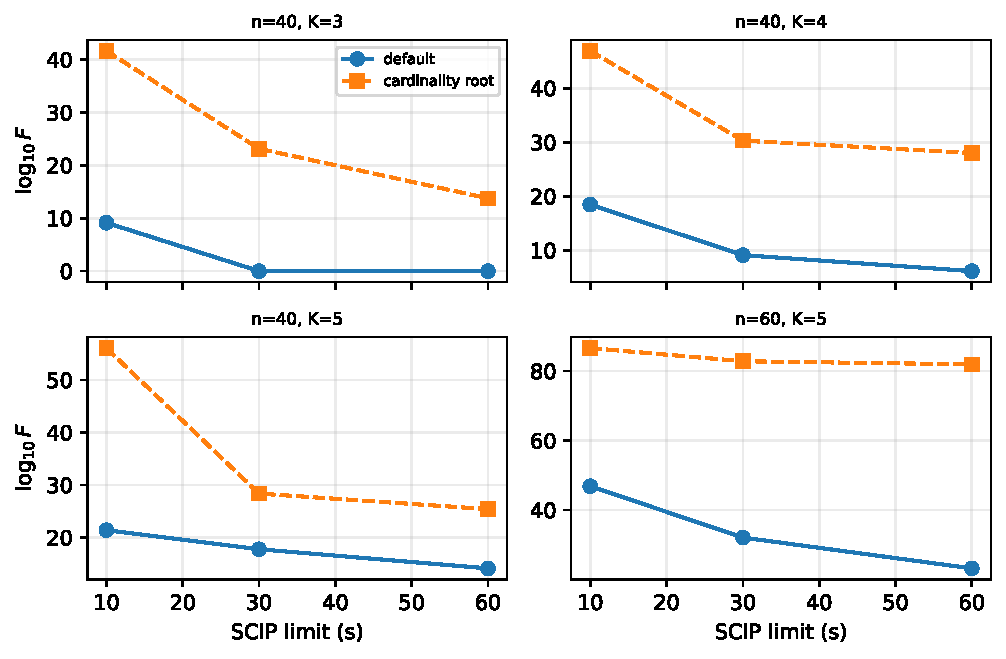
\includegraphics[width=0.85\textwidth]{fig_e12_dual_bound_profiles.pdf}
  \caption{Solver-tolerance bound-factor trajectories on representative random-matching cells. Lower values indicate tighter solver-tolerance bounds; each point is an independent bounded SCIP run.}
  \label{fig:e12-dual-bound-profiles}
\end{figure*}

\section{Gate-dependent costs versus cut count}
\label{app:countqpd}

\subsection{Controlled and algorithm-derived examples}
\label{sec:results-count}

Unweighted cut count can rank feasible plans incorrectly. Two iSWAP cuts have modeled overhead $49^2=2{,}401$, whereas three CNOT cuts cost $9^3=729$; the three-cut plan is cheaper. Likewise, two CS cuts cost $(3+2\sqrt{2})^2\approx33.97$, compared with $81$ for two CNOT cuts. Equation~\eqref{eq:weight} preserves these gate-dependent distinctions.

\begin{table}[tbp]
\centering
\caption{Identity-free heterogeneous-QPD companion corpus. All costs come from Qiskit's independent-QPD registry.}
\label{tab:heterogeneous}
\tabfit{%
\begin{tabular*}{\columnwidth}{@{\extracolsep{\fill}}lr@{}}
\toprule
\textbf{Metric} & \textbf{Value}\\
\midrule
Instances & 120 (5 families; $n\in\{12,14,16\}$)\\
Strict reversals & 16 (13.3\%)\\
Median / p90 factor & $5.30\times$ / $27.47\times$\\
Extra cuts, median / max & 1 / 3\\
Avoided iSWAP cuts & 28\\
Independent solver check closed & 120/120\\
\bottomrule
\end{tabular*}
}
\end{table}

We test this distinction under controlled heterogeneity on 120 deterministic circuits (five families, $n\in\{12,14,16\}$) using validated Qiskit costs for CX, CZ, iSWAP, and three nonzero $RZZ$ angles, with no unit-overhead operation. To avoid tie-breaking artifacts, we compare $\min_{P:\,c(P)=c^*}J(P)$, the best QPD objective among all minimum-cut partitions, with $\min_PJ(P)$; both values are obtained by exhaustive enumeration. This stronger regret is strict in $16/120$ cases ($13.3\%$), with conditional factor median $5.30$, 90th percentile $27.47$, and maximum $181.11$ (Table~\ref{tab:heterogeneous}). Every strict reversal requires more cuts under a QPD-optimal plan (median count increase one, maximum three). Across the 16 reversals, QPD-optimal plans cut 28 fewer iSWAP gates while accepting 47 additional lower-overhead gates.

We then test whether this mechanism occurs without constructed gate palettes. The algorithm-derived study uses six MQT~Bench families~\cite{mqtbench}, six even sizes, the eligibility criterion, and the decision rule before inspecting outcomes; it selectively expands only operations with arity above two, preserves numeric one- and two-qubit semantic operations, never transpiles to a target basis, and queries every retained two-qubit occurrence via \texttt{QPDBasis.from\_instruction}. The count objective $c(P)$ and QPD objective $J(P)$ define the set-level regret
\begin{equation}
  \Delta_{\mathrm{E6}} =
  \min_{P:\,c(P)=c^*} J(P) - \min_P J(P),
  \qquad c^* = \min_P c(P),
  \label{eq:e6-regret}
\end{equation}
and a strict reversal requires $\Delta_{\mathrm{E6}}>10^{-10}$. Fixing qubit zero removes complementary-label symmetry, leaving $\binom{n-1}{n/2-1}$ balanced partitions, all of which are exhaustively evaluated (from 10 at $n=6$ through $6{,}435$ at $n=16$). All 36 circuits are eligible: none has an unsupported or unit-overhead two-qubit operation, and each has at least two positive QPD-cost classes. Exhaustive optimal-set enumeration finds six strict reversals: four among six Draper QFT adders and two among six exact-QPE circuits (Table~\ref{tab:e6-summary}). HHL, inexact QPE, QFT, and entangled QFT supply 24 negative results despite heterogeneous costs. Thus heterogeneity is necessary for the observed mechanism but is not sufficient to change the optimum.

\begin{table}[tbp]
\centering
\caption{Algorithm-derived MQT~Bench audit. ``Max factor'' is descriptive over six fixed sizes per family, not a population estimate.}
\label{tab:e6-summary}
\tabfit{%
\begin{tabular*}{\columnwidth}{@{\extracolsep{\fill}}lrrr@{}}
\toprule
\textbf{Family} & \textbf{Eligible} & \textbf{Reversals} & \textbf{Max factor}\\
\midrule
Draper QFT adder & 6/6 & 4/6 & $1.04\times10^6$\\
HHL & 6/6 & 0/6 & $1$\\
Exact QPE & 6/6 & 2/6 & $4.03$\\
Inexact QPE & 6/6 & 0/6 & $1$\\
QFT & 6/6 & 0/6 & $1$\\
Entangled QFT & 6/6 & 0/6 & $1$\\
\bottomrule
\end{tabular*}
}
\end{table}

The largest observed witness is the Draper QFT adder at $n=16$: the best count-optimal plan has 36 cuts and $J=37.968133$, whereas the QPD-optimal plan has 42 cuts and $J=24.111328$, yielding a factor $1.042\times10^6$. The QPD plan avoids expensive $CP(\pi/2)$ and $CP(\pi)$ crossings by accepting more small-angle controlled phases (Table~\ref{tab:e6-draper}). Direct occurrence-level sums and independently aggregated pair weights agree within $10^{-10}$ for both plans in every reversal record. Figure~\ref{fig:draper-topology} makes the same Draper $n=16$ witness geometric: node colors encode the two fragments, while edge darkness encodes independent-QPD log weight; the count-optimal map severs fewer interactions but retains several high-$\rho$ controlled phases across the cut, whereas the QPD-optimal map accepts six additional crossings yet eliminates most expensive phase crossings. This is existence evidence on algorithm-derived benchmark circuits, not a prevalence estimate over workloads or a hardware-routing result.

\begin{figure*}[tp]
  \centering
  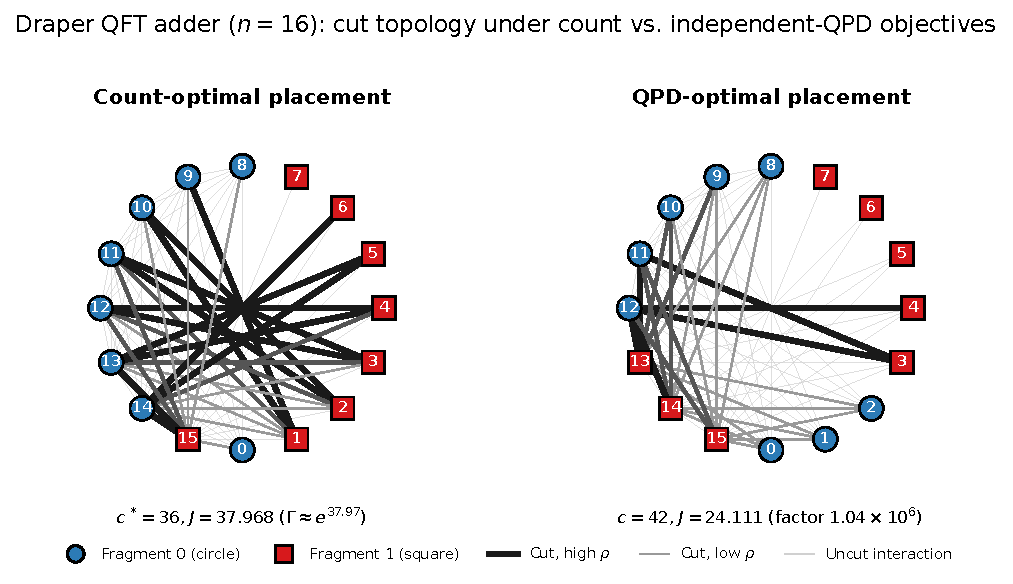
\includegraphics[width=0.85\textwidth]{fig_draper_n16_topology.pdf}
  \caption{Draper QFT-adder interaction topology at $n=16$ under exact balanced bipartition. Left: count-optimal placement ($c^*=36$, $J\approx37.97$). Right: independent-QPD-optimal placement ($c=42$, $J\approx24.11$). Darker cut edges carry larger $\log\rho$; the QPD plan trades cut count for avoidance of high-overhead controlled phases.}
  \label{fig:draper-topology}
\end{figure*}

\begin{table}[tbp]
\centering
\caption{Grouped nonzero-delta gate-class accounting for the Draper $n=16$ witness. The groups sum to $+6$ cuts and $J_{\rm QPD}^*-J_{\rm count}^*=-13.856805$; full per-angle accounting is in the reproducibility artifact.}
\label{tab:e6-draper}
\tabfit{%
\begin{tabular*}{\columnwidth}{@{\extracolsep{\fill}}lrrr@{}}
\toprule
\textbf{CP angle class} & \textbf{Count} & \textbf{QPD} & $\boldsymbol{\Delta c}$\\
\midrule
$-\pi/64$ through $-\pi/4$ & 5 & 13 & $+8$\\
$\pi/64$ through $\pi/16$ & 6 & 15 & $+9$\\
$\pi/4$ & 5 & 2 & $-3$\\
$\pi/2$ & 6 & 2 & $-4$\\
$\pi$ & 6 & 2 & $-4$\\
\midrule
Total & 28 & 34 & $+6$\\
\bottomrule
\end{tabular*}
}
\end{table}

\section{Extreme Grover representation cases}
\label{app:grover}

Five Grover records have disjoint optimal-placement sets under the two representations. These cases also exhibit very large representation expansion and correspondingly large modeled log-overheads, so they are not used as operational examples in the main text. The exact $n=10$, $K=2$ case has $\Delta_{\mathrm{CX}\to\mathrm{native}}=448.23$ and $\Delta_{\mathrm{native}\to\mathrm{CX}}=1494.11$; multiplicative factors are therefore reported in the log domain when direct exponentiation exceeds floating-point range. The largest case, at $n=16$ and $K=3$, has $\Delta_{\mathrm{CX}\to\mathrm{native}}=9984.19$ ($\log_{10}R=4336.1$), with $234{,}300$ and $395{,}044$ two-qubit gate occurrences in the CX-normalized and native representations, respectively. The corresponding optimum log-objectives are $J_a^*=240244.5$ and $J_b^*=394375.4$, while $\|\delta\|_1=371287.2$. The regret is therefore about $2.7\%$ of the total interaction-weight perturbation. We report $\log_{10}R=\Delta/\ln 10$ directly for these cases to avoid numerical overflow. The $n=16$, $K=2$ Grover record is also present and has $R=1$ under the set-level comparison.

\section{Additional optimization scaling results}
\label{app:scaling}

\subsection{Capacitated \texorpdfstring{$K$}{K}-way heterogeneous scaling}
\label{app:scaling-detail}

\begin{table*}[t]
\centering
\caption{Capacitated $K$-way heterogeneous-QPD scaling, three fixed seeds per cell and a 10-s SCIP limit. ``Closed'' means solver-tolerance closure. Open records retain finite factors, including $10^{43.48}$ at random-matching $n=60,K=4$; this fixed matrix is not a workload-prevalence estimate.}
\label{tab:e9-kway}
\tabfitstar{%
\begin{tabular*}{\textwidth}{@{\extracolsep{\fill}}lccc@{}}
\toprule
\textbf{Family} & \textbf{Closed} & \textbf{All-seed closure frontier} & \textbf{Boundary}\\
\midrule
Random matching & 24/48 & $K=2,n=60;\,K=4,n=20$ & $K\geq3,n\geq40$\\
Community matching & 37/48 & $K=3,n=60;\,K=4,n=40$ & $K=5,n\geq32$\\
Weighted repeat & 40/48 & $K=3,n=60;\,K=4,n=40$ & $K\geq4,n=60$\\
\midrule
Total & 101/144 & $n=60,K=3$ & family/seed dependent\\
\bottomrule
\end{tabular*}
}
\end{table*}

\begin{table*}[t]
\centering
\caption{Matched-objective baseline results. Regret statistics use 101 solver-tolerance-closed records only. A method matches on a record when $|\log_{10}R|\le10^{-10}$. KaHIP time includes an unbounded native call and is not budget matched ($\dagger$).}
\label{tab:e9-heuristic}
\tabfitstar{%
\begin{tabular*}{\textwidth}{@{\extracolsep{\fill}}lrrrrrr@{}}
\toprule
\textbf{Method} & \textbf{Feasible} & \textbf{Match / closed} & \textbf{Med. $\Delta J$} & \textbf{Med. $\log_{10}R$} & \textbf{p90 $\log_{10}R$} & \textbf{Med. time}\\
\midrule
Greedy swap & 144/144 & 23/101 & 3.33 & 1.45 & 10.52 & 0.100 s\\
Count-KL & 144/144 & 23/101 & 3.59 & 1.56 & 5.01 & 0.100 s\\
KL-QPD & 144/144 & 68/101 & 0.00 & 0.00 & 2.94 & 0.100 s\\
KaHIP+repair & 144/144 & 51/101 & 0.00 & 0.00 & 1.47 & 5.89 s$^\dagger$\\
\bottomrule
\end{tabular*}
}
\end{table*}

We evaluate the core formulation~\eqref{eq:kway} beyond bisection on a heterogeneous-QPD benchmark of 144 runs (three fixed seeds per family--size--$K$ cell, $n\le60$, $K\le5$, 10-s SCIP limit). Table~\ref{tab:e9-kway} and Fig.~\ref{fig:e9-closure} summarize all runs, including open cases. SCIP reaches solver-tolerance closure on $101/144$ runs. The boundary is strongly graph- and seed-dependent: community matching and weighted repeat close all three seeds through $(K,n)=(3,60)$ and $(4,40)$, whereas random matching is the hard family---all three $K=2,n=60$ runs close, but every $K\geq3,n\geq40$ run remains open.

The factors quantify why closure alone is insufficient. Across the three random-matching $n=32,K=5$ runs, the median open factor is $10^{15.47}$; at $n=60,K=4$ it is $10^{43.48}$. The latter is deliberately prominent: it is an extreme resource-risk bound, not a near-optimality result. These values state that the corresponding incumbents carry no useful solver-tolerance multiplicative overhead guarantee at this deadline, and their explicit reporting prevents an unproven incumbent from being presented as an optimum. Thus this study establishes a practical baseline and a transparent computational boundary, not universal large-$K$ scalability. A tighter-tolerance sensitivity rerun of 24 matched seed-0 instances spanning 24 benchmark cells at \texttt{numerics/feastol}$=10^{-9}$ (SCIP~10.0.2, seed~0) leaves every closed/open classification unchanged relative to the original \texttt{feastol}$=10^{-6}$ runs and reproduces each jointly closed log-objective with no observed difference at the recorded numerical precision, confirming that within this sensitivity subset all classifications are stable under the tighter feasibility tolerance. The exact-capacity comparison also expresses the fragment-width/overhead tradeoff directly: increasing $K$ reduces the maximum fragment size while generally forcing more independent-QPD boundaries (Fig.~\ref{fig:e9-pareto}).

We further confirm that cut count is a poor proxy for sampling overhead at the placement level using matched-objective heuristics that solve the same fixed independent gate-QPD, exact-capacity $K$-way problem: greedy swap, a count-weighted pairwise Kernighan--Lin (KL) adaptation, QPD-weighted KL, and KaHIP-QPD with exact-capacity repair~\cite{kernighanlin1970,kahip}. One canonical evaluator recomputes $J$, fragment sizes, and cut occurrences for every method, and also re-evaluates each reported SCIP incumbent after decoding it to a discrete partition. On the 101 solver-tolerance-closed records (Table~\ref{tab:e9-heuristic}), KL-QPD matches the SCIP objective on 68 records with median $\log_{10}R=0$ and p90 $2.94$, whereas count-weighted KL matches only 23 with median $\log_{10}R=1.56$; the two differ only in objective semantics within one heuristic family, isolating the effect of optimizing overhead rather than count. All 144 partitions from every matched method satisfy exact capacities. We also apply the same native independent-QPD model to 36 algorithm-derived MQT~Bench circuits: SCIP closes 15 within 10~s, KL-QPD matches all 15 solver-tolerance-closed objectives, and the six Draper-adder records form the largest structured positive subset. Three VQE candidates are retained as explicit ingestion failures because their native two-qubit operations lack a Qiskit QPD basis. Thus the heuristic finding is not solely a synthetic-graph artifact.

\begin{figure*}[tp]
  \centering
  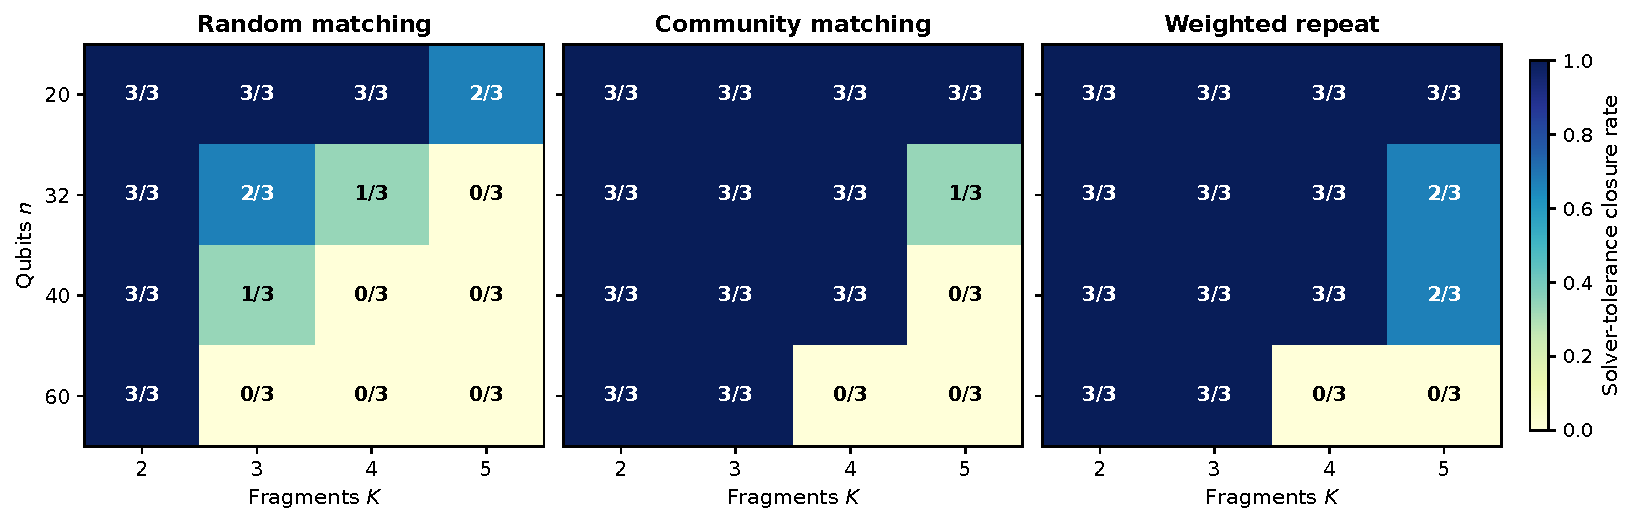
\includegraphics[width=0.85\textwidth]{fig_e9_closure_heatmap.pdf}
  \caption{Solver-tolerance closure counts under a 10-s SCIP limit. Each heatmap cell reports closed runs out of three fixed seeds. The boundary depends materially on graph family, $K$, and seed.}
  \label{fig:e9-closure}
\end{figure*}

\begin{figure}[tbp]
  \centering
  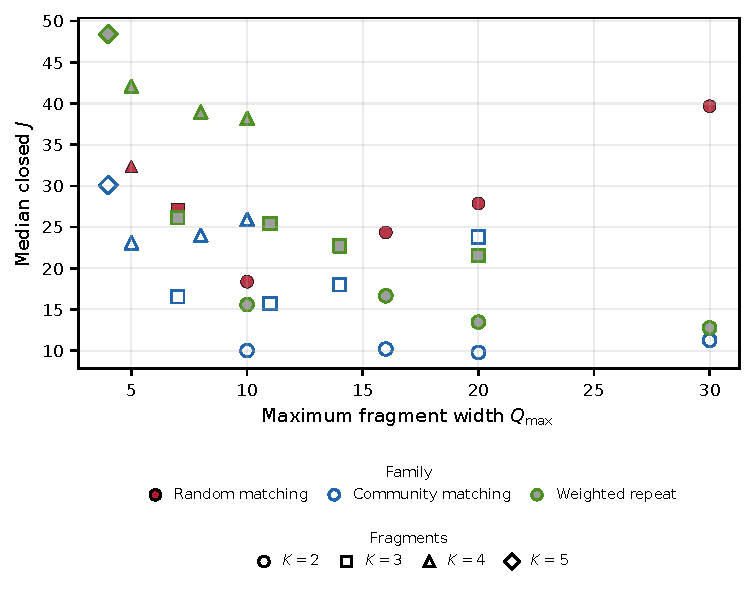
\includegraphics[width=\columnwidth]{fig_e9_width_overhead_pareto.pdf}
  \caption{Width--overhead tradeoff restricted to cells closed for all three seeds. Colors denote families, with distinct fill treatments (filled, open, gray-filled) so that families remain distinguishable in grayscale; markers denote $K$. Each point is the median solver-tolerance-closed log-objective $J$ for its cell.}
  \label{fig:e9-pareto}
\end{figure}

\section{Resource-model sensitivity and finite-shot tests}
\label{app:scope}

\subsection{Sensitivity to the quasiprobability resource model}
\label{sec:results-joint}

Independent QPD is a declared cut-cost model, not an assertion that stronger joint decompositions preserve placements. We therefore test whether the optimal placement can itself depend on the assumed resource model. Under a restricted library of pairwise-disjoint same-layer gate groups, a controlled six-qubit witness makes the independent-QPD-optimal placement $1.90496\times$ worse than the restricted-joint optimum when both are evaluated under the restricted parallel-joint semantics: a model-induced placement reversal exists. This is the resource-model analogue of the representation reversals of Sec.~\ref{sec:results-reversals}---there the interaction weights change because the gate-level representation changes; here they change because the assumed decomposition changes---and it shows that the placement decision is a function of the declared resource model as well as of the circuit.

We then test algorithm-derived native-QPD circuits under the same restricted pair library. The joint-aware MIP matches exhaustive enumeration on all 17 records with $n\le12$ and finds no strict independent-to-joint reversal in that subset, despite eligible saving opportunities. The experiment is limited to this restricted pair library; general joint-QPD-aware partitioning, together with wire-cut and hybrid gate/wire models, remains future work~\cite{schmitt2025,ufrecht2024,brenner2025}.

\subsection{Finite-shot scope}
\label{sec:results-shot}

A final study fixes an equal total ideal-Aer shot budget on three $n=12$ witnesses. The strong $719.66\times$ modeled reversal reduces RMSE for both observables, whereas a moderate $3.27\times$ reversal is mixed and a no-reversal control is identical under shared seeds. Hence independent-QPD overhead can be operationally informative but is not claimed as a universal finite-shot RMSE predictor. Full witness identities, signed-estimator behavior, and bootstrap intervals remain in the artifact. This study evaluates finite-shot behavior in an ideal-simulator implementation rather than modeling it.

\section{Verified interval tier and reconstruction check}
\label{app:verified}

To ground the word ``certificate'' in a rigorously verified setting, a small CX-only tier is certified using exact interval arithmetic rather than SCIP bounds. It exhaustively enumerates 20 exact-input balanced-bipartition records with 80-decimal directed intervals for $\log 9$: nine have a uniquely separated optimum, and the remaining records certify the optimum objective in the presence of ties. Interval widths are $2\times10^{-79}$ to $3\times10^{-78}$, so these optima are numerical proofs up to verified outward rounding, not solver-tolerance estimates. This is the only tier for which we use certificate in the strong sense; it is an enumerative interval oracle that verifies objective values independently but does not verify production SCIP lower bounds.

Independently, a shot-free statevector reconstruction check (Table~\ref{tab:operational}) confirms that predicted and Qiskit-derived overheads agree at machine precision, validating the cost accounting used throughout.

\begin{table}[tbp]
\centering
\caption{Statevector reconstruction check. Predicted and Qiskit-derived overheads agree; ``Abs. error'' compares reconstructed and uncut observables.}
\label{tab:operational}
\tabfit{%
\begin{tabular*}{\columnwidth}{@{\extracolsep{\fill}}lcccc@{}}
\toprule
\textbf{Circuit} & \textbf{Cuts} & \textbf{Pred. $\Gamma$} & \textbf{Exec. $\Gamma$} & \textbf{Abs. error}\\
\midrule
QAOA $n\!=\!6$, native $RZZ$ & 2 & 33.9706 & 33.9706 & $1.39\!\times\!10^{-17}$\\
VQE $n\!=\!6$, CX             & 1 & 9       & 9       & $5.55\!\times\!10^{-17}$\\
\bottomrule
\end{tabular*}
}
\end{table}

\FloatBarrier

% ===================================================================
% REFERENCES
% ===================================================================
\bibliography{references}

\end{document}
